% chapters/chapter1.tex  — converted from chapter1.typ
% Conventions used:
%   Typst @KEY            -> \ac{KEY}        (auto: long on first use, short after)
%   Typst @KEY:pls        -> \acsp{KEY}      (short plural, e.g. "AVs")
%   Typst @KEY:pla        -> \acp{KEY}       (auto plural)
%   Typst @KEY:l          -> \acf{KEY}       (forced full form "Long (SHORT)")
%   Typst @KEY:lo         -> \acl{KEY}       (long form only)
%   Typst @figlabel       -> Figure~\ref{fig:figlabel}
%   Typst @citekey        -> \cite{citekey}
% Inside captions \acs{} is used so float placement cannot disturb first-use timing.

\chapter{Introduction}
\label{ch1}

\section{What is autonomous driving}
For 3 million years human beings have been creating tools to ease their daily chores in order to make a better life. One of the successful creations of humans as a decent invention is vehicles. The first automobile ever created dates to the late 19th century. Since then vehicles have been evolving rapidly, so in recent decades we have had a new concept of vehicle, so-called \enquote{\ac{AV}}.

\acsp{AV}, or self-driving cars, are vehicles as discussed earlier that can ease human daily driving tasks by taking them one by one to do them themselves.

\acsp{AV} represent the next major step in the evolution of road transportation, extending earlier advances in vehicle automation and driver assistance systems. As sensing, computing power, and control technologies have matured, vehicles have gained the ability to monitor their surroundings, interpret complex traffic situations, and support or even replace human driving tasks. Early prototypes in the 1980s and 1990s, enabled by progress in computer vision, robotics, and embedded systems, demonstrated that vehicles could follow lanes, maintain speed, and avoid obstacles under constrained conditions. The parallel development of GPS-based positioning, digital mapping, and onboard sensors such as cameras, radars, and lidars provided the foundation for modern perception systems. In the last 7 decades, autonomous driving has seen big advances which can be seen in Figure~\ref{fig:historical_development}. These technological advances collectively enabled the transition from basic driver assistance toward higher levels of automation, where vehicles can execute steering, acceleration, and braking tasks with increasing independence from human input. Driverless vehicle technology gained momentum at the beginning of the 21st century. Initiatives like Google's driverless car project~\cite{waymo-self-cars} captured public attention and created a general awareness that autonomous driving was a real possibility. The use of cameras, radars, lidars, and artificial intelligence algorithms in vehicles endowed them with the capability to navigate complex traffic situations independently. Many car manufacturers and technology companies are now accelerating their efforts to develop fully \acp{AV}. The goal of these vehicles is to reduce traffic accidents, increase transportation efficiency, and provide greater independence for people with mobility limitations. However, technical challenges, as well as ethical, legal, and safety issues, continue to shape the advancement in this field. The future of autonomous driving depends on overcoming these challenges and gaining societal acceptance for this new technology.

\section{Importance of Simulation in Autonomous Driving}
\begin{figure}[htbp]
    \centering
    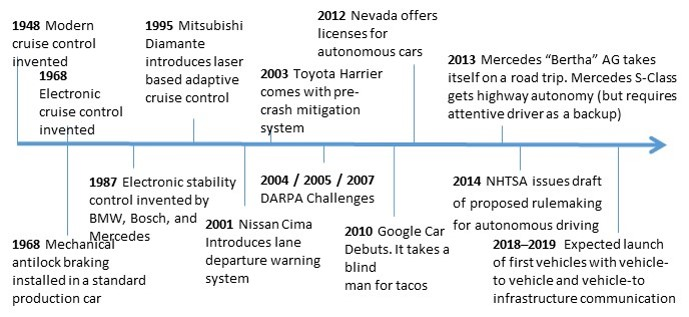
\includegraphics{image/Historical development of autonomous driving.jpeg}
    \caption{The historical development of autonomous driving~\cite{inbook}.}
    \label{fig:historical_development}
\end{figure}

In today's world, developing and using software has become very important across many industries. While these software solutions provide us with numerous conveniences and advantages, they also introduce certain requirements. One of the most critical requirements for any software is testing. The testing phase can be used to determine whether an application fulfills its intended function or to assess its efficiency. Of course, in some sectors, this functionality takes on an even greater importance. One such area is safety. In industries like aviation and automotive, where a user's safety can be directly affected by an error in the application, testing and simulation are more important than ever. In model-based software applications, after a model is created, it moves to the verification stage. Before being loaded onto the hardware, the model undergoes several verification steps (as the V-model in Figure~\ref{fig:v_model}). Some of these verifications are named \ac{MIL}~\cite{plummer-2006}, \ac{SIL}~\cite{4455268}, and \ac{HIL}~\cite{fathy-2006}.

\textbf{\acs{MIL}} In the initial stages of system design, before real hardware or software components are implemented, the simulation and testing of system models are carried out by the \ac{MIL} testing method. This method uses mathematical models and simulations for system or component design. These models are utilized to understand how the designed system will function and behave. \ac{MIL} testing is a critical tool for verifying the design and identifying potential problems at an early stage. With this method, engineers and designers can gain valuable insights into how the system will operate before actually manufacturing the hardware or fully developing the software.

\textbf{\acs{SIL}} The \ac{SIL} testing method is the process of testing a system or component's software without using real hardware. This method simulates environmental factors or other parts interacting with the system while the software runs directly on a computer. This simulation evaluates the software's behavior and performance under real-world conditions. The main goal of \ac{SIL} testing is to verify the software's functionality, detect errors at an early stage, and analyze interactions between the system and the software. This approach accelerates the software development and refinement processes and prevents costly errors.

\textbf{\acs{HIL}} The \ac{HIL} testing method creates an environment to control and test real hardware. In this method, the hardware being tested, such as a vehicle control unit, operates in real time, but the software simulates the physical systems (e.g., engines, sensors, actuators, etc.) interacting with the hardware in real time. This simulation allows for the evaluation of how the hardware performs under real-world conditions.

\begin{figure}[htbp]
    \centering
    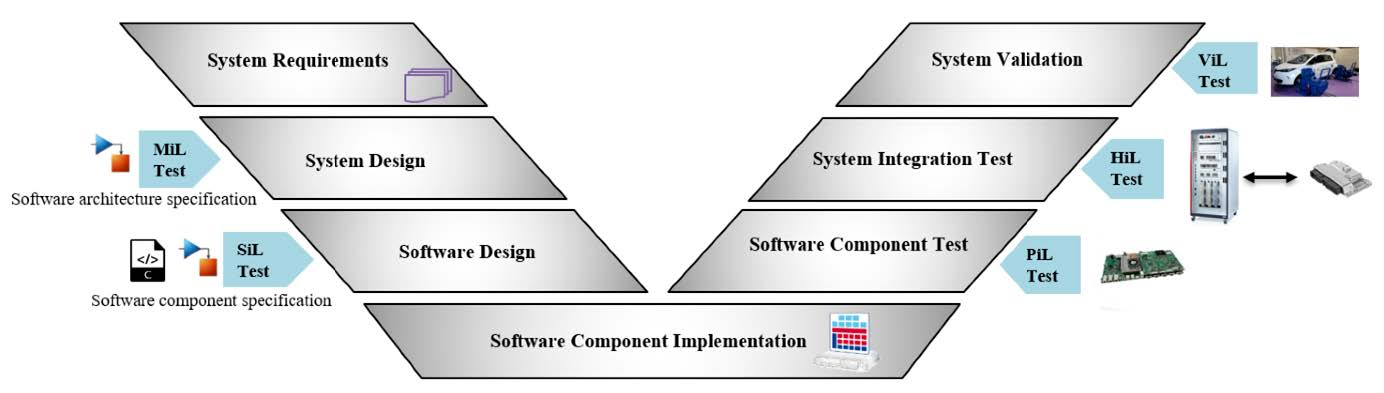
\includegraphics{image/v cycle development process.jpeg}
    \caption{\acs{MIL}, \acs{SIL}, PIL, \acs{HIL} and \acs{VIL} tests in the V-cycle development process~\cite{article}.}
    \label{fig:v_model}
\end{figure}

In Figure~\ref{fig:driving_test_simulator} a driving test simulator is shown. Test simulators typically fall under the \ac{SIL} category. The \ac{SIL} testing method has numerous advantages. These benefits explain why \ac{SIL} tests are an important part of the software development process and demonstrate their value to engineers and developers across various industries. The main advantages can be listed as follows:

\textbf{Cost Efficiency:} \ac{SIL} tests are conducted in a simulated environment that does not require real hardware, thus reducing the costs associated with purchasing, maintaining, and repairing hardware. Additionally, early diagnosis of potential errors helps prevent more costly problems later on.

\textbf{Rapid Feedback Loop:} Testing software in a model allows for quick iterations in the development process. This enables developers to instantly see the effects of their code and make fast modifications if necessary.

\textbf{Risk Reduction:} Tests conducted without real hardware use a simulated environment to safely examine situations that could be potentially dangerous or harmful to the hardware. This is especially important when expensive hardware is involved.

\textbf{Broad Test Scenarios:} \ac{SIL} tests are capable of quickly and easily testing a wide range of scenarios that mimic real-world conditions. Developers can experiment with system parameters, error states, and various operational conditions.

\textbf{Acceleration of the Development Process:} \ac{SIL} tests can speed up the development process instead of waiting for the hardware to be ready. Testing the software alongside hardware development shortens the time to market for the product.

\textbf{Preparation for Integration and System Tests:} When software is successfully tested in a \ac{SIL} environment, the transition to more complex testing stages where hardware and software are run together becomes easier. This helps reduce problems that may arise during system tests and integration.

\begin{figure}[htbp]
    \centering
    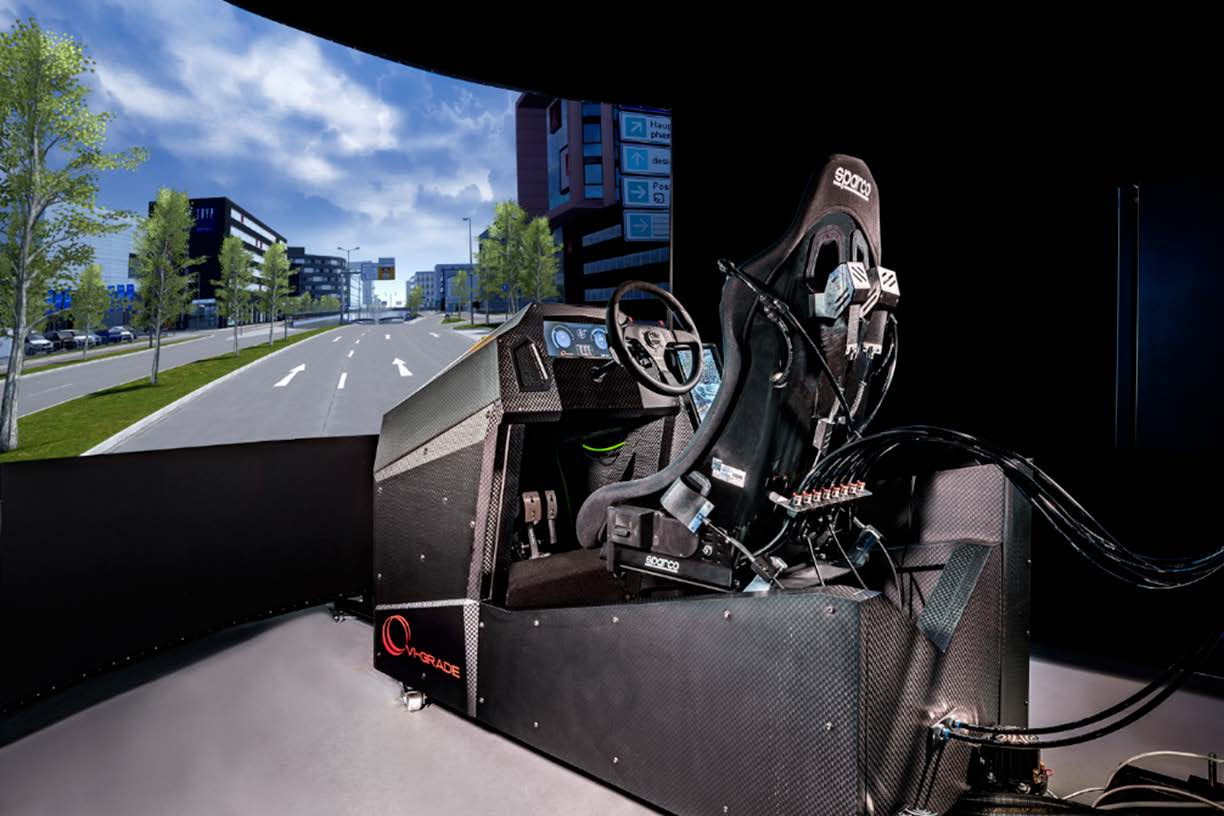
\includegraphics{image/driving test simulator.jpeg}
    \caption{Driving test simulator~\cite{Sim}.}
    \label{fig:driving_test_simulator}
\end{figure}

\textbf{Flexibility in the Development Process:} Software can be tested and developed with various hardware platforms and configurations. This flexibility allows for the evaluation of how the software will perform on different systems.

\section{State of the Art in Autonomous Driving Simulators}
Advancements in the field of autonomous driving have also led to the development of powerful autonomous driving simulators. Nowadays, a wide range of simulators produced by various companies are in use. These include open-source projects (e.g.\ CARLA~\cite{dosovitskiy-2017}, AirSim~\cite{shah-2017}), commercial software, and customized simulation solutions used in academic and industrial research. In the context of this thesis, a simulation environment is essential, because the \acf{LKA} function is developed and evaluated entirely in a virtual \ac{VIL} setup rather than on a physical test vehicle. Therefore, it is crucial to clearly define the requirements that the simulator must satisfy---such as realistic sensor models, controllable traffic and weather, and reproducible scenarios---and to justify the choice of a specific platform.

In the following, I first review several popular autonomous driving simulation tools and platforms available in the literature and in practice. The comparison focuses on criteria such as graphic quality, accuracy of the physics engine, sensor simulation capabilities, simulation of traffic and pedestrians, weather conditions, and the ability to simulate at different times of the day. Based on these criteria, I motivate the selection of CARLA as the main simulation platform for this work and explain how it will be used to implement and test the proposed \ac{LKA} function.

\subsection{Waymo simulator}
\begin{figure}[htbp]
    \centering
    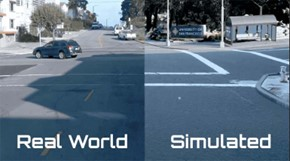
\includegraphics{image/waymo real world comparison.jpeg}
    \caption{Comparing Waymo Simulator graphics and the real world.}
    \label{fig:waymo}
\end{figure}
Waymo possesses an advanced simulation platform~\cite{gulino2023waymaxaccelerateddatadrivensimulator} and is widely recognized as a leader in \ac{AV} technology. This simulator plays a crucial role in the development and testing of autonomous driving systems by providing a highly realistic (as can be seen in Figure~\ref{fig:waymo}) and comprehensive virtual environment. It combines high-fidelity graphics that accurately replicate real-world environments with a precise physics engine capable of modeling vehicle dynamics, collisions, and surface interactions. Furthermore, it includes detailed sensor emulation for LIDAR, radar, and cameras, enabling a realistic representation of environmental perception. The platform can also model complex traffic flow and pedestrian behaviors, which are essential for evaluating \acsp{AV} in dense urban settings. In addition, the simulator supports a wide range of weather and lighting conditions, allowing performance assessment under rain, snow, fog, or low-light scenarios. Owing to these capabilities, the Waymo simulator holds a significant position among state-of-the-art autonomous driving simulation platforms.

\subsection{SVL Simulator}
\begin{figure}[htbp]
    \centering
    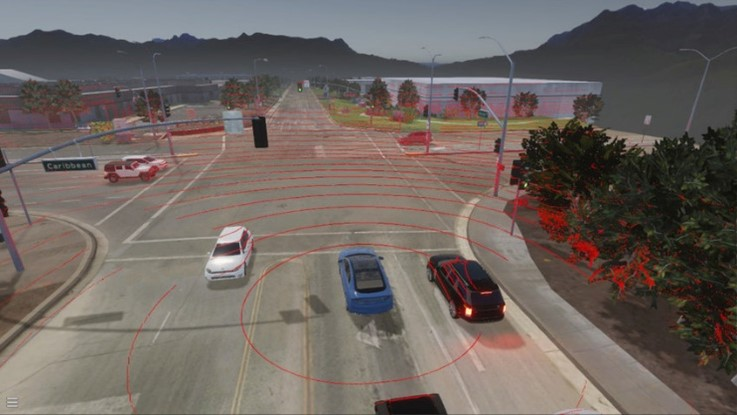
\includegraphics{image/svl screen.jpeg}
    \caption{SVL Simulator Screen.}
    \label{fig:svl}
\end{figure}
The \ac{AV} research community frequently employs the LGSVL Simulator~\cite{rong2020lgsvlsimulatorhighfidelity}, an open-source platform designed for high-fidelity testing of perception and control algorithms. Thanks to its Unity-based rendering engine, LGSVL offers realistic visual environments suitable for evaluating camera-based functions. Its physics engine provides detailed modeling of vehicle dynamics, tire--road interactions, and collisions, enabling credible closed-loop testing of control algorithms. The simulator includes configurable sensor models---such as lidar, radar, and cameras---along with comprehensive traffic and pedestrian behavior, allowing researchers to model complex urban scenarios (Figure~\ref{fig:svl}). Furthermore, LGSVL supports diverse weather and lighting conditions, which makes it valuable for assessing the robustness of autonomous driving functions under varying environmental circumstances. LGSVL represents an important reference point when comparing available simulation platforms.

\subsection{Sim4CV}
\begin{figure}[htbp]
    \centering
    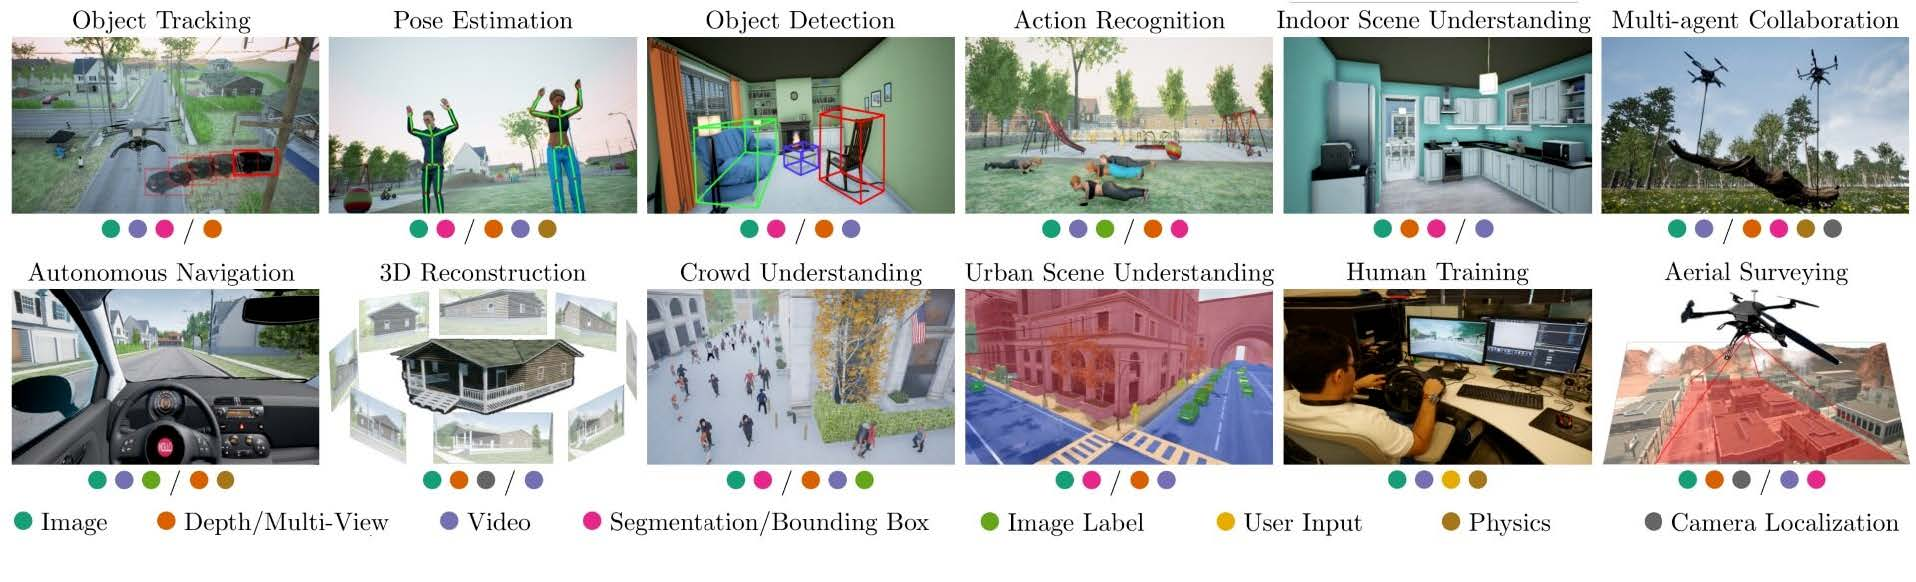
\includegraphics{image/sim4cv.jpeg}
    \caption{Sim4CV: A Photo-Realistic Simulator for Computer Vision Applications.}
    \label{fig:sim4sv}
\end{figure}
Sim4CV is a simulation platform developed for research in computer vision and autonomous systems, with a strong emphasis on autonomous driving and aerial navigation~\cite{muller-no-date}. Built on Unreal Engine 4, it provides high-quality visual environments and a physics engine capable of modeling realistic vehicle dynamics, object interactions, and environmental effects. The platform supports the simulation of various sensors, including cameras and lidar, enabling detailed testing of perception algorithms. Sim4CV also offers traffic and pedestrian simulation, though the level of sophistication may vary across versions and configurations (Figure~\ref{fig:sim4sv}). Furthermore, the ability to adjust weather and lighting conditions makes it suitable for evaluating algorithm robustness under diverse environmental scenarios.

\subsection{CARLA Simulator}
\begin{figure}[htbp]
    \centering
    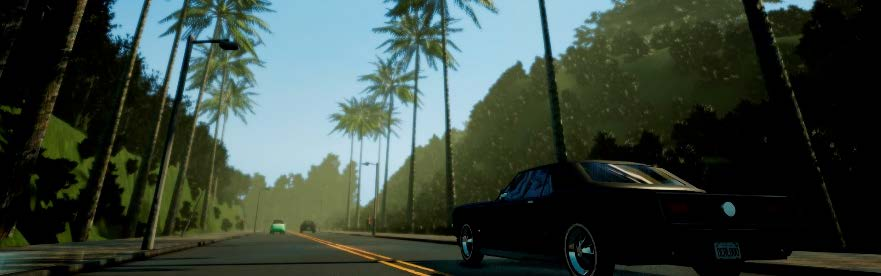
\includegraphics{image/carla screen2.jpeg}
    \caption{CARLA Simulator Screen.}
    \label{fig:carla_screen}
\end{figure}
The CARLA Simulator is an open-source autonomous driving platform~\cite{team-no-date} widely used in research for developing, testing, and validating \ac{AV} algorithms. Built on Unreal Engine 4, it provides high-fidelity graphics that closely resemble real-world environments (Figure~\ref{fig:carla_screen}), which is essential for evaluating perception systems. The underlying physics engine of CARLA accurately models vehicle dynamics, collisions, and surface interactions, enabling realistic assessment of control and planning algorithms. It also offers comprehensive sensor simulation---including cameras, LIDAR, radar, and GNSS---allowing researchers to replicate and analyze diverse sensing conditions. In addition, CARLA supports dynamic traffic scenarios and human-like pedestrian behavior, creating complex and socially interactive environments for autonomous driving studies. Finally, its configurable weather and lighting system makes it possible to test algorithms across various environmental conditions, ensuring robustness and generalizability in real-world deployments.

\begin{table}[htbp]
    \centering
    \footnotesize
    \begin{tabular}{@{}p{4.6cm}cccc@{}}
        \hline
        Features / Simulators & Waymo & LGSVL & Sim4CV & CARLA \\
        \hline
        Graphics Quality                     & 8/10 & 9/10 & 8/10 & 9/10 \\
        Physics Engine Accuracy              & 8/10 & 9/10 & 7/10 & 9/10 \\
        Sensor Simulation                    & 8/10 & 9/10 & 7/10 & 9/10 \\
        Traffic and Pedestrian Simulation    & 8/10 & 9/10 & 6/10 & 9/10 \\
        Weather Conditions                   & 7/10 & 8/10 & 6/10 & 9/10 \\
        Simulation at Different Times of Day & 7/10 & 8/10 & 6/10 & 9/10 \\
        \hline
    \end{tabular}
    \caption{Comparative Feature Scoring of Simulators.}
    \label{tab:simulators}
\end{table}
Using a set of predefined evaluation criteria---such as graphics quality, physics realism, sensor simulation, traffic modeling, and environmental variability---a comparative score was assigned to each simulator. Table~\ref{tab:simulators} summarizes the evaluation results based on these criteria.

\section{ADAS Applications}
\ac{ADAS} are becoming increasingly common in today's vehicles. Developed to enhance vehicle safety and the driving experience, these systems utilize various technologies such as cameras, sensors, and radars to identify potential hazards and are designed to alert the driver or automatically control the vehicle under certain conditions. \acs{ADAS} technologies not only assist drivers in traveling more safely and comfortably but also have the potential to reduce traffic accidents. There are various applications of \acs{ADAS}, which are crucial for the safety of the driver and also provide significant conveniences. Some of these applications can be briefly discussed as follows:

\begin{wrapfigure}{r}{0pt}
    \centering
    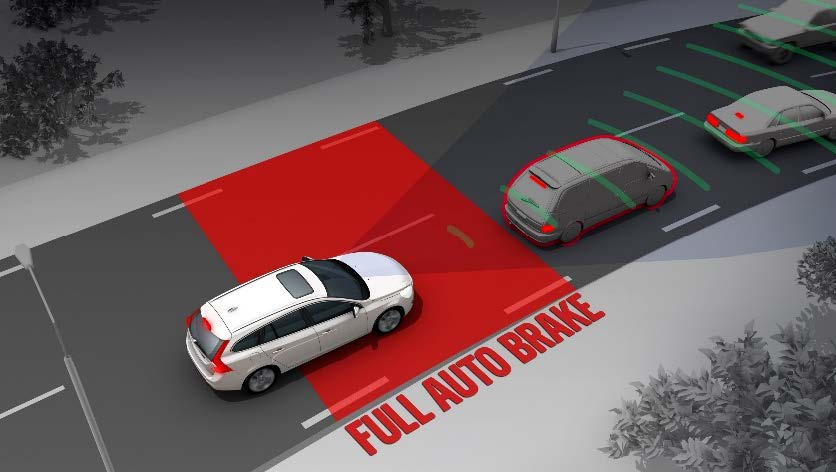
\includegraphics{image/emergency braking.jpeg}
    \caption{Automatic Emergency Braking system.}
    \label{fig:emergency_breaking}
\end{wrapfigure}

\textbf{Automatic Emergency Braking:} The vehicle automatically brakes to avoid colliding with a vehicle or obstacles ahead~\cite{5625077}. A laser radar sensor detects the distance to the vehicle ahead and the relative speed. If there is an object in the area seen by the laser radar sensor at this speed, the brakes are activated to prevent a collision as shown in Figure~\ref{fig:emergency_breaking}. Additionally, in some vehicles, it works in conjunction with seat belts activated by braking before a collision to help reduce injuries in cases where a collision is unavoidable.

\begin{wrapfigure}{l}{0pt}
    \centering
    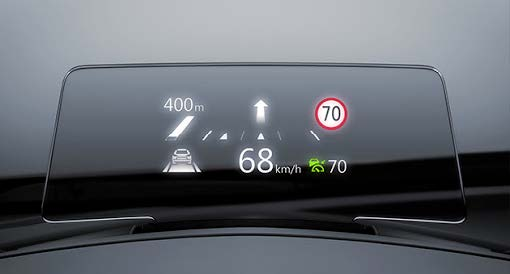
\includegraphics{image/traffic sign.jpeg}
    \caption{Traffic Sign Recognition System.}
    \label{fig:traffic}
\end{wrapfigure}

\textbf{Traffic Sign Recognition System:} This system detects traffic signs and informs the driver about traffic rules such as speed limits and prohibition signs. Generally, an image is captured by a camera sensor placed on the vehicle's windshield, and the detected image is projected onto the user's screen (Figure~\ref{fig:traffic}). This technology aims to prevent accidents by ensuring that drivers do not overlook important warning signs on the road~\cite{fu-2010}.

\begin{wrapfigure}{r}{0pt}
    \centering
    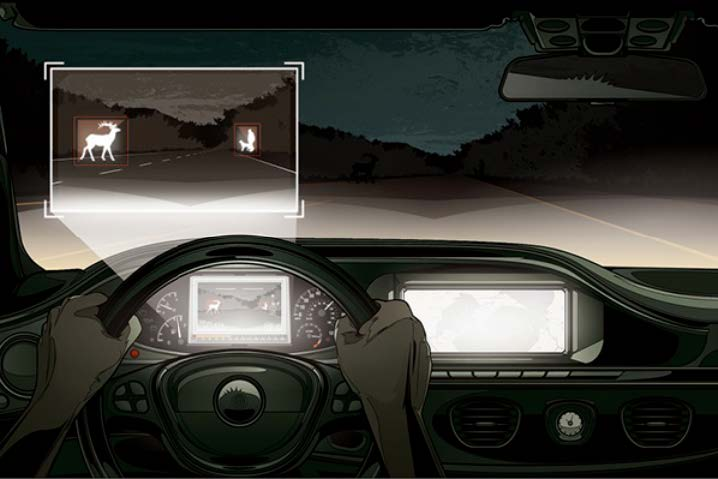
\includegraphics{image/night vision.jpeg}
    \caption{Night Vision.}
    \label{fig:Night}
\end{wrapfigure}

\textbf{Night Vision:} This system expands the driver's field of vision in low-light conditions or at night through cameras or other sensors~\cite{kupper-2002}. Utilizing thermal cameras and infrared lights, it detects living beings on the road ahead and provides audible or visual warnings to the driver (Figure~\ref{fig:Night}). In addition to detection, advanced night vision systems can highlight potential hazards directly on the dashboard display or head-up display.

\begin{wrapfigure}{l}{0pt}
    \centering
    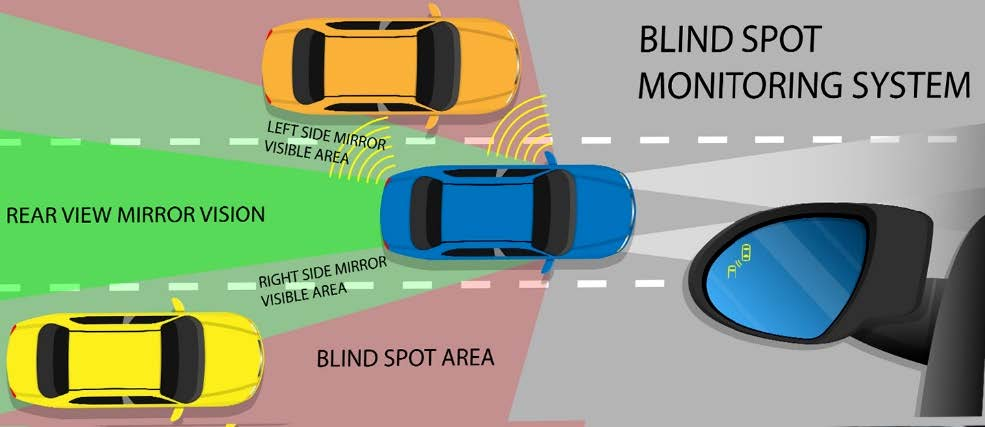
\includegraphics[width=0.5\textwidth]{image/blind spot.jpeg}
    \caption{Blind Spot Warning System.}
    \label{fig:blind_spot}
\end{wrapfigure}

\textbf{Fatigue Detection Systems:} Various studies have suggested that approximately 20\% of all road accidents, and up to 50\% on certain roads, are fatigue-related~\cite{wikipedia-contributors-2025}. Although the implementation of this system varies among manufacturers, some brands warn the driver by detecting steering movements and how often the vehicle drifts out of its lane.

\textbf{Blind Spot Warning System:} This system identifies the presence of other vehicles in the vehicle's blind spots and informs the driver about them. Vehicles in the blind spot are detected using radar sensors located on the sides of the rear bumper (Figure~\ref{fig:blind_spot}). A warning is displayed to the driver in the side mirror, and if the driver signals to change lanes while there is a vehicle in the blind spot, an alert is issued. In some models, changing lanes by braking is prevented to enhance the safety of the driver in the car and to avoid road accidents~\cite{liu-2017}.

\begin{wrapfigure}[11]{r}{0pt}
    \centering
    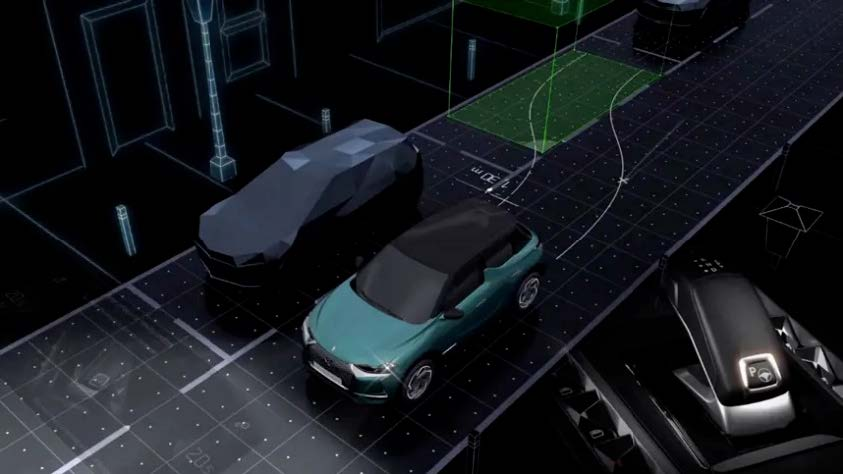
\includegraphics{image/parking assistant.jpeg}
    \caption{Parking Assistant.}
    \label{fig:parking_assist}
\end{wrapfigure}

\textbf{Parking Assistant:} This feature assists the driver in better positioning the vehicle while parking and, in some cases, can automatically park the vehicle (Figure~\ref{fig:parking_assist}). It utilizes parking sensors located around the vehicle to do this~\cite{7548171}. Parking sensors are generally electromagnetic sensors. Commonly, the system is used in a manner where the driver is still responsible for commands such as gas and gear changes.

\begin{wrapfigure}{l}{0pt}
    \centering
    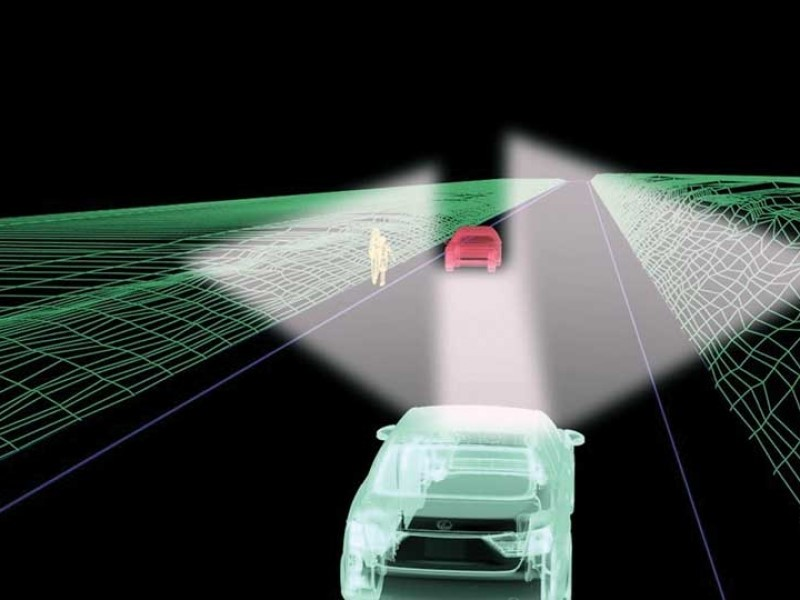
\includegraphics{image/automatic headlight control.jpeg}
    \caption{Automatic Headlight Control.}
    \label{fig:automatic_headlight}
\end{wrapfigure}

\textbf{Automatic Headlight Control:} The effectiveness of vehicle headlights becomes even more crucial on roads with insufficient external lighting at night, such as forest roads. Oncoming drivers on these types of roads can be affected by the headlight beams. Systems like this reduce the light intensity when detecting an oncoming vehicle to minimize the adverse effects on the opposite driver. In more advanced models, the direction of the headlight beam is adjusted to achieve this effect (Figure~\ref{fig:automatic_headlight}).

\begin{wrapfigure}{r}{0pt}
    \centering
    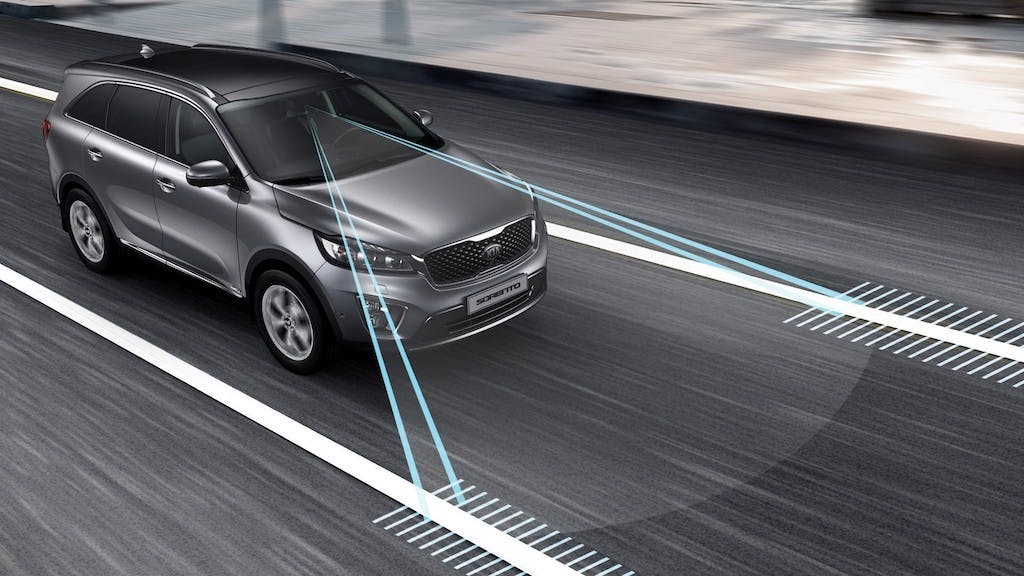
\includegraphics{image/lane keeping.jpeg}
    \caption{\acs{LKA} demonstration.}
    \label{fig:lane_keeping_assist}
\end{wrapfigure}

\textbf{\acl{LKA}:} This system uses a camera sensor to detect the distance of the vehicle from the lane markings and activates when the determined distance falls below a certain threshold (Figure~\ref{fig:lane_keeping_assist}). It steers the steering wheel to direct the vehicle back into the lane, ensuring it remains within its lane boundaries. It acts as a countermeasure to unintentional drifting, reducing relevant accidents by over 20\%.

\begin{wrapfigure}{l}{0pt}
    \centering
    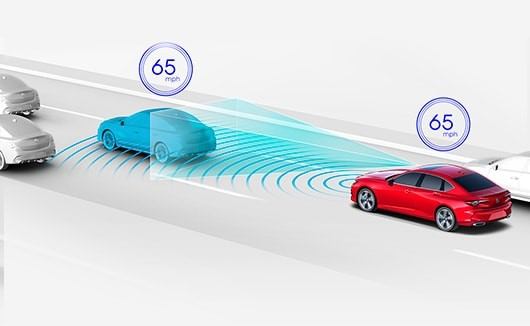
\includegraphics{image/acc.jpeg}
    \caption{Adaptive Cruise Control.}
    \label{fig:adaptive_cruise}
\end{wrapfigure}

\textbf{Adaptive Cruise Control:} This system is a more advanced version of the traditional cruise control system~\cite{my-car-does-what-2018}. While traditional cruise control maintains the vehicle at a set speed, this system adapts the speed based on the speed of the vehicle ahead (Figure~\ref{fig:adaptive_cruise}). It utilizes two separate sensors to accomplish this. The first sensor is a radar sensor that measures the distance to the vehicle in front. The second sensor is a speed sensor that detects any decrease or increase in the vehicle's speed. Based on the information from these sensors, decisions are made and implemented to accelerate or decelerate. Generally, the desired distance and following speed can be adjusted by the user via controls on the steering wheel.

\section{Related Works}
The research community has proposed various methods for validating autonomous driving functions using simulation and \ac{VIL} concepts, as well as a wide range of lateral control strategies for path and lane tracking. This section summarizes the most relevant works and explains how they relate to the present thesis, which implements a \ac{LKA} function in the CARLA simulator using an external Python-based controller and an RGB camera.

\paragraph{\acs{VIL} simulation}
Son et al.\ propose a PG-based \ac{VIL} simulation framework that combines a real vehicle with a virtual driving environment for system development and consistency validation~\cite{electronics11244073}. Their system includes modules for virtual road generation, synchronization between real and virtual domains, a virtual traffic manager, and perception sensor modelling. They demonstrate that the behavior observed in the \ac{VIL} simulation setup is consistent with physical vehicle tests over different speeds, road types, and surrounding environments. This work shows how \ac{VIL} can improve reproducibility and safety when testing autonomous driving systems.

Cheng et al.\ provide a comprehensive survey on testbench-based Vehicle-in-the-Loop simulation testing for \acsp{AV}~\cite{survey_test_bench}. They review existing \ac{AV} testing approaches and identify limitations of traditional methods. The paper then focuses on testbench-based \ac{VIL} architectures, principles, and equipment, with particular emphasis on physical signal stimulation and realistic road condition simulation. The survey identifies research gaps between current testbench technologies and industrial \ac{AV} testing needs, and highlights \ac{VIL} as a promising tool for accurate and efficient validation.

Xiong Hu et al.\ present a \ac{VIL} simulation test framework for \acsp{AV}, where an autonomous driving system is evaluated using a virtual environment combined with real vehicle components~\cite{xiong_hu}. Their work emphasizes the synchronization of vehicle dynamics and simulated scenarios and discusses how \ac{VIL} can be used to test autonomous driving functions safely and systematically.

These works clearly show that \ac{VIL} is an important methodology for validating autonomous driving systems. However, they mainly focus on general architectures, testbench setups, and system-level validation. They do not specifically address a software-only \ac{VIL} configuration in a driving simulator like CARLA, where a simulated vehicle is controlled by external code using RGB camera images. Furthermore, the detailed design and evaluation of a single \acs{ADAS} function such as \ac{LKA}---implemented and tested entirely in such a \ac{VIL} setup---remains less explored. This is where the present thesis contributes.

\paragraph{Lateral control for \acsp{AV}}
Lateral control is a key component for lane keeping and path tracking. Kebbati et al.\ provide a technical review of lateral control methods for autonomous wheeled vehicles~\cite{kebbati}. They classify control approaches into model-based and data-driven methods, and discuss their advantages, limitations, and implementation challenges. The survey underlines that lateral control must deal with accuracy, robustness, and real-time constraints, and highlights open challenges for future research.

Artu\~{n}edo et al.\ present a comparative evaluation of state-of-the-art lateral control strategies for \acsp{AV}~\cite{ARTUNEDO2024100910}. They propose a systematic tuning methodology and define a comprehensive set of performance metrics covering tracking accuracy, robustness, and comfort. The controllers are evaluated in extensive simulations and real-vehicle tests over different trajectories and scenarios. Their results show how different control strategies behave under the same conditions and provide guidance for selecting suitable lateral controllers.

Dominguez et al.\ experimentally compare several classical lateral controllers---such as Pure Pursuit and Stanley---on an \ac{AV} platform~\cite{7795743}. They study the performance of these controllers in terms of tracking error and stability, using a combination of simulation and real-world experiments. Their work provides practical insight into the behavior of commonly used path-tracking controllers and their suitability for autonomous driving applications.

Snider's technical report is a widely cited reference on automatic steering methods for autonomous automobile path tracking~\cite{Snider2009AutomaticSM}. It describes the mathematical formulation and implementation details of several steering controllers, including Pure Pursuit and Stanley, and discusses their application to \acsp{AV}. This report is frequently used as a theoretical foundation when implementing classical lateral control laws.

These studies provide a solid theoretical and experimental basis for the lateral control part of \ac{LKA}. However, most of them either assume ideal path or lane information (for example, predefined waypoints or ground-truth lane geometry) or focus on real-vehicle experiments without an explicit simulation-based \ac{VIL} framework. They do not analyze in detail how classical lateral controllers perform when they receive lane information from a real-time camera-based perception pipeline inside a simulator.

\paragraph{Identified gap and relation to this thesis}
In summary, the literature on \ac{VIL} shows how combined real--virtual setups can be used to validate autonomous driving systems~\cite{electronics11244073, survey_test_bench, xiong_hu}, while the lateral control literature provides a variety of controllers and comparative evaluations for path and lane tracking~\cite{kebbati, ARTUNEDO2024100910, 7795743, Snider2009AutomaticSM}. However, the combination of these two aspects,
\begin{itemize}
    \item a \textbf{\acs{VIL}-style simulation environment} in a high-fidelity simulator, and
    \item a \textbf{camera-based \acs{LKA} function} implemented as an external control stack,
\end{itemize}
is less represented in the existing works.

The present thesis addresses this gap by implementing a modular \ac{LKA} system in CARLA, where an RGB camera provides input to an external Python program that estimates lane geometry and computes steering commands. The system is evaluated in a reproducible simulation environment, thus connecting the ideas of \ac{VIL}-based validation and classical lateral control within a single, integrated \ac{LKA} framework.
